\documentclass[11pt,a4paper]{article}
\usepackage{fullpage}	% Bigger pages
\usepackage{cite} 		% Include citations
\usepackage{hyperref} 	% Hyperlinks everywhere!
\usepackage{natbib}		% Include bibliography
\usepackage{graphicx}	% Include pictures
\usepackage{amsmath}	% Use \eqref

\begin{document}

\title{Constraining the Hemispherical Structure in the Hidden Layer At the Top of the Earth's Inner Core}
\author{Candidate Number: \\  \\ Supervisor: Prof. Keith Priestley}
\maketitle

\begin{abstract}
Since its discovery in 1936, the Earth's inner core has been well documented by both body wave and normal mode studies. However, one area where properties are not yet well measured is the top of the inner core. The upper region of the inner core is of particular interest as it is thought that as the outer core freezes onto the inner core the variable environment at this boundary is encoded in the properties of the frozen material. 
\end{abstract}

\tableofcontents

\newpage
\section{Introduction}
The inner core was first discovered by Inge Lehmann in 1936, who used the existence of P wave arrivals within the P wave shadow zone to infer a solid-liquid boundary lying within the core mantle boundary (\cite{Lehmann}). Over the following 80 years large progress has been made on measuring the properties of the inner core, but there is much still to learn.

Of particular interest is the velocity and attenuation structure, which can be used to infer the chemical and physical properties of the inner core's constituent material. The following gives a summary of these properties, and is quoted directly from \cite{Deuss2014}:
\begin{itemize}
	\item The top 60-80 km of the inner core is isotropic, and the deeper parts have 3-4\% anisotropy. The anisotropy exists in both velocity and attenuation; waves traveling in the polar direction are faster and more attenuated than waves traveling equatorially.
	\item There may be an innermost inner core with different anisotropy, though evidence is not compelling.\footnote{Research published since \cite{Deuss2014} provides strong evidence for this (\cite{Wang2015}).}
	\item The inner core displays a hemispherical variation: The western hemisphere is more strongly anisotropic, has a lower isotropic compressional velocity, and is less attenuating than the eastern hemisphere. There are sharp boundaries between the two hemispheres.
	\item Inner core superrotation is less than $0.5^{\circ}$ /yr and may even be as small as $0.1-1^{\circ}$ /Myr.
\end{itemize}

The upper inner core is of particular interest, as material from the outer core is currently freezing onto it at a rate of around 1mm/year (\cite{Labrosse2001}). Modelling performed by \cite{Deguen2009a} shows that the velocity structure of the upper inner core should reflect recent processes in the lower upper core. Thus measuring the structure of the upper inner core could in turn give insights into areas such as how the outer core generates the Earth's magnetic field. 

So far only large scale velocity structures have been measured, with the most recent velocity models BEING VERY COARSE GRAINED. In addition the extent to which the methodology used here and elsewhere is not well understood. In this paper we tackle both of these problems.

We do so by taking individual earthquakes that travel to multiple seismic stations and identifying the arrival of distant seismic phases in seismograms. We constrain our analysis to the uppermost inner core as far as is possible, and area not yet investigated in published literature.

Section \ref{sec:Theory} gives an brief theoretical background, with section \ref{sec:Data} describing our data collection and pre-processing. Waveform analysis is discussed in section \ref{sec:Waveforms} leading to regional velocity model results presented in section \ref{sec:Models}.

%%%
\section{Theoretical Background}
\label{sec:Theory}
We use seismic body wave analysis in order to investigate the velocity structure of the upper inner core. These waves elastic waves, caused by earthquakes, that travel through the interior of the Earth.

\subsection{Body Wave Theory}
Here we summarise the main aspects of seismic body wave theory, taken from \cite{Shearer2009}.

Under the assumptions of a continuous, linearly elastic medium, infinitesimal strains and constant medium properties one can derive the elastic wave equation
\begin{equation}
	\rho \frac{\partial^{2} \vec{u}}{\partial t^{2}} = \left ( \lambda + \mu \right ) \nabla \left ( \nabla \cdot \vec{u} \right ) + \mu \nabla^{2} \vec{u}
	\label{eq:Wave Equation}
\end{equation}
where u is the local displacement vector, $\rho$ the density of the medium and $\lambda$ and $\mu$  Lam\'{e} parameters of the medium. A general displacement vector can be decomposed into irrotational scalar and solenoidal vector potentials such that
\begin{equation}
	u \equiv \nabla \phi + \nabla \times \vec{\psi}
	\label{eq:Displacement}
\end{equation}
Substituting \eqref{eq:Displacement} in to \eqref{eq:Wave Equation} yields two independent wave equations, one for $\phi$ and one for $\vec{\psi}$, which describe P-waves and S-waves respectively. P-waves are compressional with displacements occurring parallel to the wave vector, whereas S-waves are transverse with displacements occurring perpendicular to the wave vector. These wave equations take the form
\begin{equation}
	\frac{\partial^{2} \phi}{\partial t^{2}} = c^{2} \left ( \vec{x} \right ) \nabla^{2} \phi
\end{equation}
where $c(\vec{x})$ is the local wave velocity that depends on position. A velocity model is a full specification of $c(\vec{x})$ in the region of interest.

\subsection{Sampling the Inner Core}
\label{sec:Sampling}
Because the outer core is liquid with $\mu \approx 0$ and thus does not transmit S-waves, it is P-waves that are used to sample the inner core. Figure PUT FIGURE HERE shows the ray path for the PKiKP and PKIKP phase; they travel almost identical paths through the Crust, Mantle and upper Outer Core, after which PKiKP reflects off the Inner Core boundary, whereas PKIKP travels just underneath the boundary in the Inner Core.

All measurements are compared to the radially symmetric global velocity model from \cite{Kennett1995b} (hereafter called AK135), from which we seek to measure perturbations about. The residual travel time CHECK ME is defined after \cite{Waszek2011a} as
\begin{equation}
	\delta t = \left ( t_{PKiKP} - t_{PKIKP} \right )_{observed} -  \left ( t_{PKiKP} - t_{PKIKP} \right )_{model}
	\label{eq:Residual definition}
\end{equation}
This equation can be reformulated as an integral along the ray paths
\begin{equation}
		\delta t = \left (  \int \frac{1}{v_{obs}} - \frac{1}{v_{model}} ds  \right )_{PKiKP} - \left (  \int \frac{1}{v_{obs}} - \frac{1}{v_{model}} ds \right )_{PKIKP}
		\label{eq:deltat}
\end{equation}
where the path to be integrated along is indicated by the subscript outside the brackets, and in general the velocities vary as a function of position.

As the inner core has a very low viscosity (eg. \cite{Wijs1998}, \cite{Zhang2000}) we assume that it is unable to sustain any long term non-radial variations in velocity structure. Under this assumption $v_{jobs} = v_{model}$ for the outer core, setting the first integral in \eqref{eq:deltat} to zero.

Taking perturbations about the model of the form $v_{obs} = v_{model} + \delta v$ gives
\begin{equation}
	\delta t =\left ( \int \frac{\delta v}{v_{model} + \delta v }\frac{1}{v_{model}} ds \right )_{PKIKP}
\end{equation}
For depths below the Inner Core boundary of less than 50km $v_{model}$ is constant for AK135, and we assume $\delta v$ is also a constant such that we are measuring only the average velocity perturbation along the ray path. We are thus left with the equation (to first order in $\delta t$) that will allow us to compute $\delta v$
\begin{equation}
	\delta v = \frac{\delta t}{t} v_{model}
	\label{eq:Delta v}
\end{equation}
where $t$ is the time PKIKP spends in the inner core. A positive residual implies a positive velocity perturbation and vice versa, as expected from equation \eqref{eq:Residual definition}.

If instead we wish to construct a layered model, we simply apply the above results to the uppermost layer, and then take the effect of the new layer into account when calculating the properties of subsequent lower layers.

%%%
\section{Data Selection}
\label{sec:Data}
As discussed in section \ref{sec:Sampling}, we make differential travel time measurements of PKiKP and PKIKP phases. An ideal seismogram would have a clear PKIKP arrival, little noise and no interference from surface reflection phases. As such, individual events are selected to meet the following criteria:

\begin{itemize}
	\item Epicentral distance of $115^{\circ}$ - $143^{\circ}$ covers the majority of North America, where there is the highest worldwide density of seismometers.
	\item  Depth greater than 15km, to minimise possible interference between PKIKP (PKiKP) and pPKIKP (pPKiKP) phases\footnote{The preceding 'p' denotes a reflection from the Earth's surface.}.
	\item Magnitude greater than 5.2 and less than 6.3 to ensure a large enough earthquake to produce an observable signal, whilst a small enough earthquake such that the rupture is likely to be impulsive.
	\item A fracture mechanism that is primarily dip slip\footnote{This means a large component of motion is in the vertical direction}. As the ray paths are themselves nearly vertical when they reach the seismic stations (see PUT RAYPATH FIGURE HERE), a significant amount of energy is required to be focused in the vertical direction at the site of the earthquake.
\end{itemize}

Individual earthquakes meeting this criteria typically contain 100 to 600 individual seismograms. Each seismogram is filtered between 0.7Hz - 2Hz in order to focus on the expected frequency of $\sim$1Hz whilst removing unwanted noise at other frequencies. Individual seismograms are then checked by hand, and only those showing a clear PKIKP signal near the predicted arrival time are kept for further analysis. Event parameters are looked up using the Central Moment Tensor (CMT) Catalogue (\cite{Dziewonski1981}, \cite{Ekstrom2012}).

%%%%
\section{Initial data analysis}
\label{sec:Waveforms}
The same analysis was performed on each individual event. Each event is listed in table \ref{tab:Events}.
\begin{table}\footnotesize
\centering
\begin{tabular}{| l | c | c | c | c | c | c |}
	\hline Location				& Latitude		& Longitude	& Date		& Time		& Magnitude	& Depth (km) 	\\ \hline
	\hline Tanzania				& -9.50		& 39.22		& 2010/08/03	& 19:42:18	& 5.3			& 32.8		\\
	\hline Banda Sea			& -7.24		& 129.83		& 2013/08/12	& 00:53:45	& 6.1			& 105.2		\\
	\hline Celebes Sea			& 4.55		& 122.82		& 2014/04/16	& 04:28:20	& 5.8			& 575.0  		\\ 
	\hline South Sandwich Islands 	& -60.01		& -26.76		& 2014/12/28	& 20:30:58	& 5.2			& 124.4		\\
	\hline	
\end{tabular}
\caption{Event details taken directly from the CMT Catalogue. Dates are formatted as year/month/day format and times as hour:minute:second}
\label{tab:Events}
\end{table}
Here we describe the analysis using data from the Celebes Sea event.

Synthetic waveforms are computed using the WKBJ ray tracing program (\cite{Chapman1976}) combined with rupture mechanisms from the CMT catalogue\footnote{See appendix \ref{app:Software} for full details of software used in our analysis.}. Predicted ray paths and individual ray travel times are computed using the TauP toolkit (\cite{Crotwell1999}). Initial plots are shown for both real and synthetic data in figures \ref{fig:Real nonaligned} and \ref{fig:Synth nonaligned} respectively, with zero time occurring at the time of the earthquake, taken from the global CMT catalogue. Overplotted are theoretical PKIKP and PKiKP travel times computed using the AK135 model (\cite{Kennett1995b}). The predicted travel times agree well with the data in both cases.  For shorter epicentral distances the predicted arrival times become closer, suggesting that eventually there will be a phase separation below which the two distinct phases will not be individually observable.

CHANGE THESE FIGURES
\begin{figure}
	\centering
	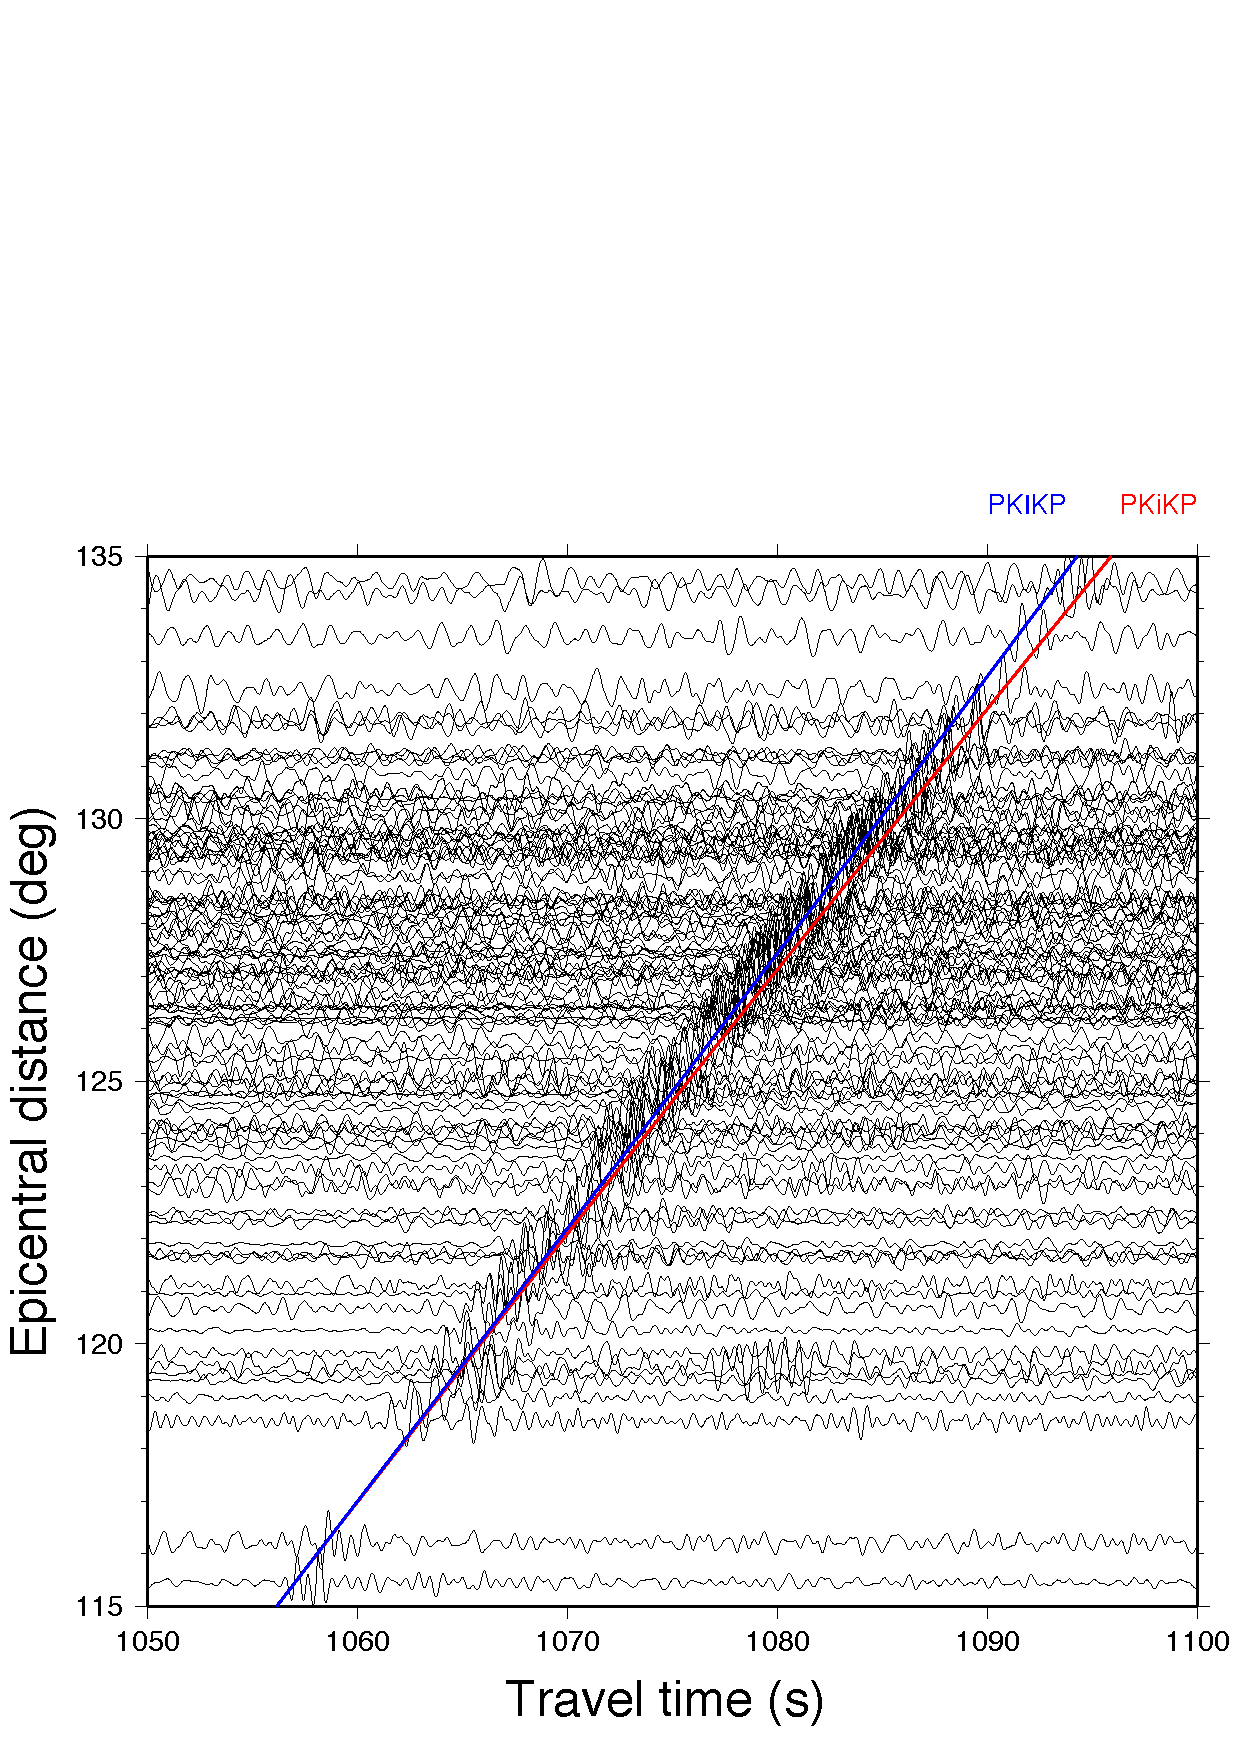
\includegraphics[width=0.6\textwidth]{figures/celebessea/celebessea_real.pdf}
	\caption{Real seismogram data from the Celebes Sea event after event selection. Each seismogram is zeroed on the earthquake time. Over plotted lines are theoretical phase arrivals computed using the AK135 model. Only data with a clear PKIKP arrival are plotted}
	\label{fig:Real nonaligned}
\end{figure}

\begin{figure}
	\centering
	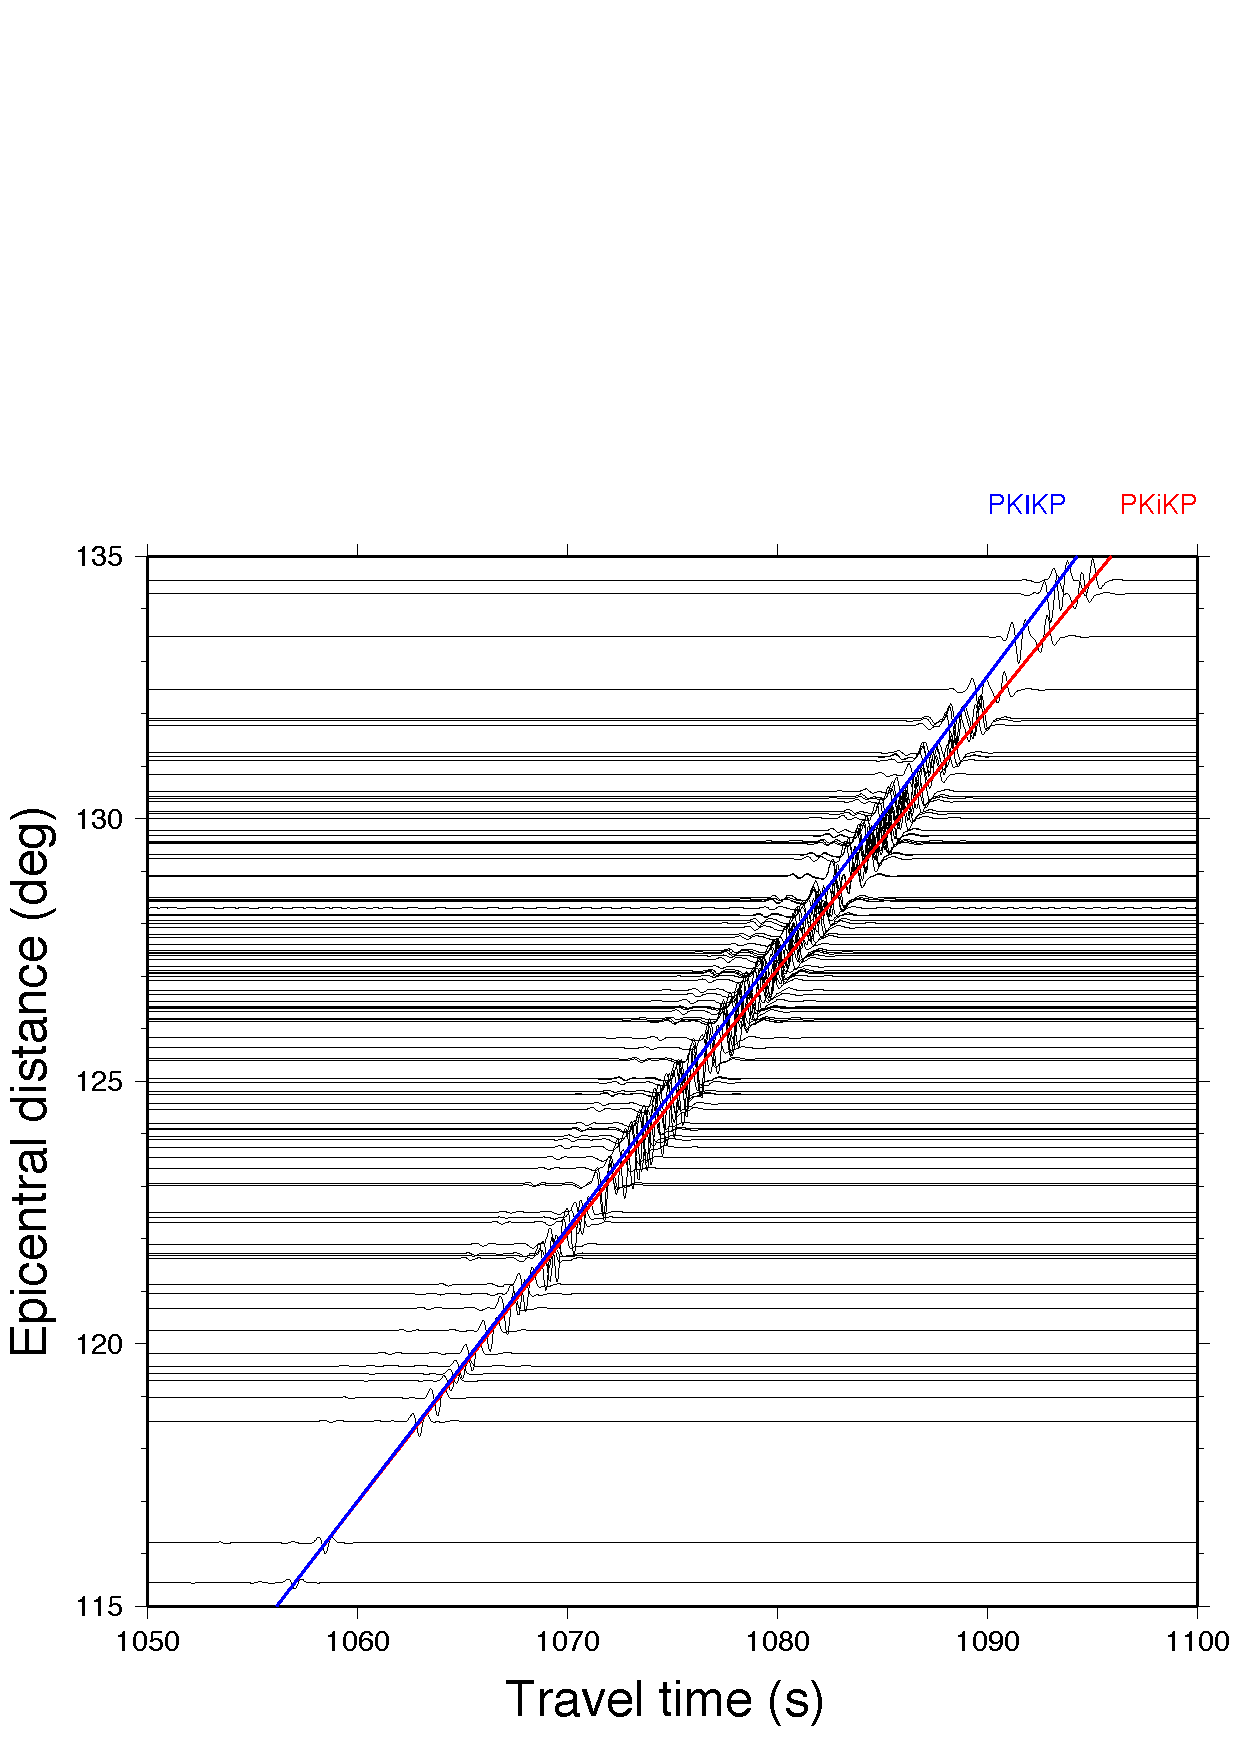
\includegraphics[width=0.6\textwidth]{figures/celebessea/celebessea_synthetic_both.pdf}
	\caption{Synthetic seismogram data for the Celebes Sea event.. Each seismogram is zeroed on the earthquake time. Over plotted lines show theoretical phase arrivals computed using the AK135 model.}
	\label{fig:Synth nonaligned}
\end{figure}

In order to more easily visualise the two phases we plot seismograms with individual PKiKP and PKIKP phases. In conjunction we also plot synthetic seismograms with both phases present, called `combined' seismograms from now on. This seismogram simulates the real world where both phases are present.

Each of these is shifted such that the initial PKIKP downswing occurs at zero time. This is shown in figure \ref{fig:Synth aligned}. It is now clear to see the PKiKP phase merging with the PKIKP phase at low epicentral distances in the combined seismogram.

\begin{figure}
	\centering
	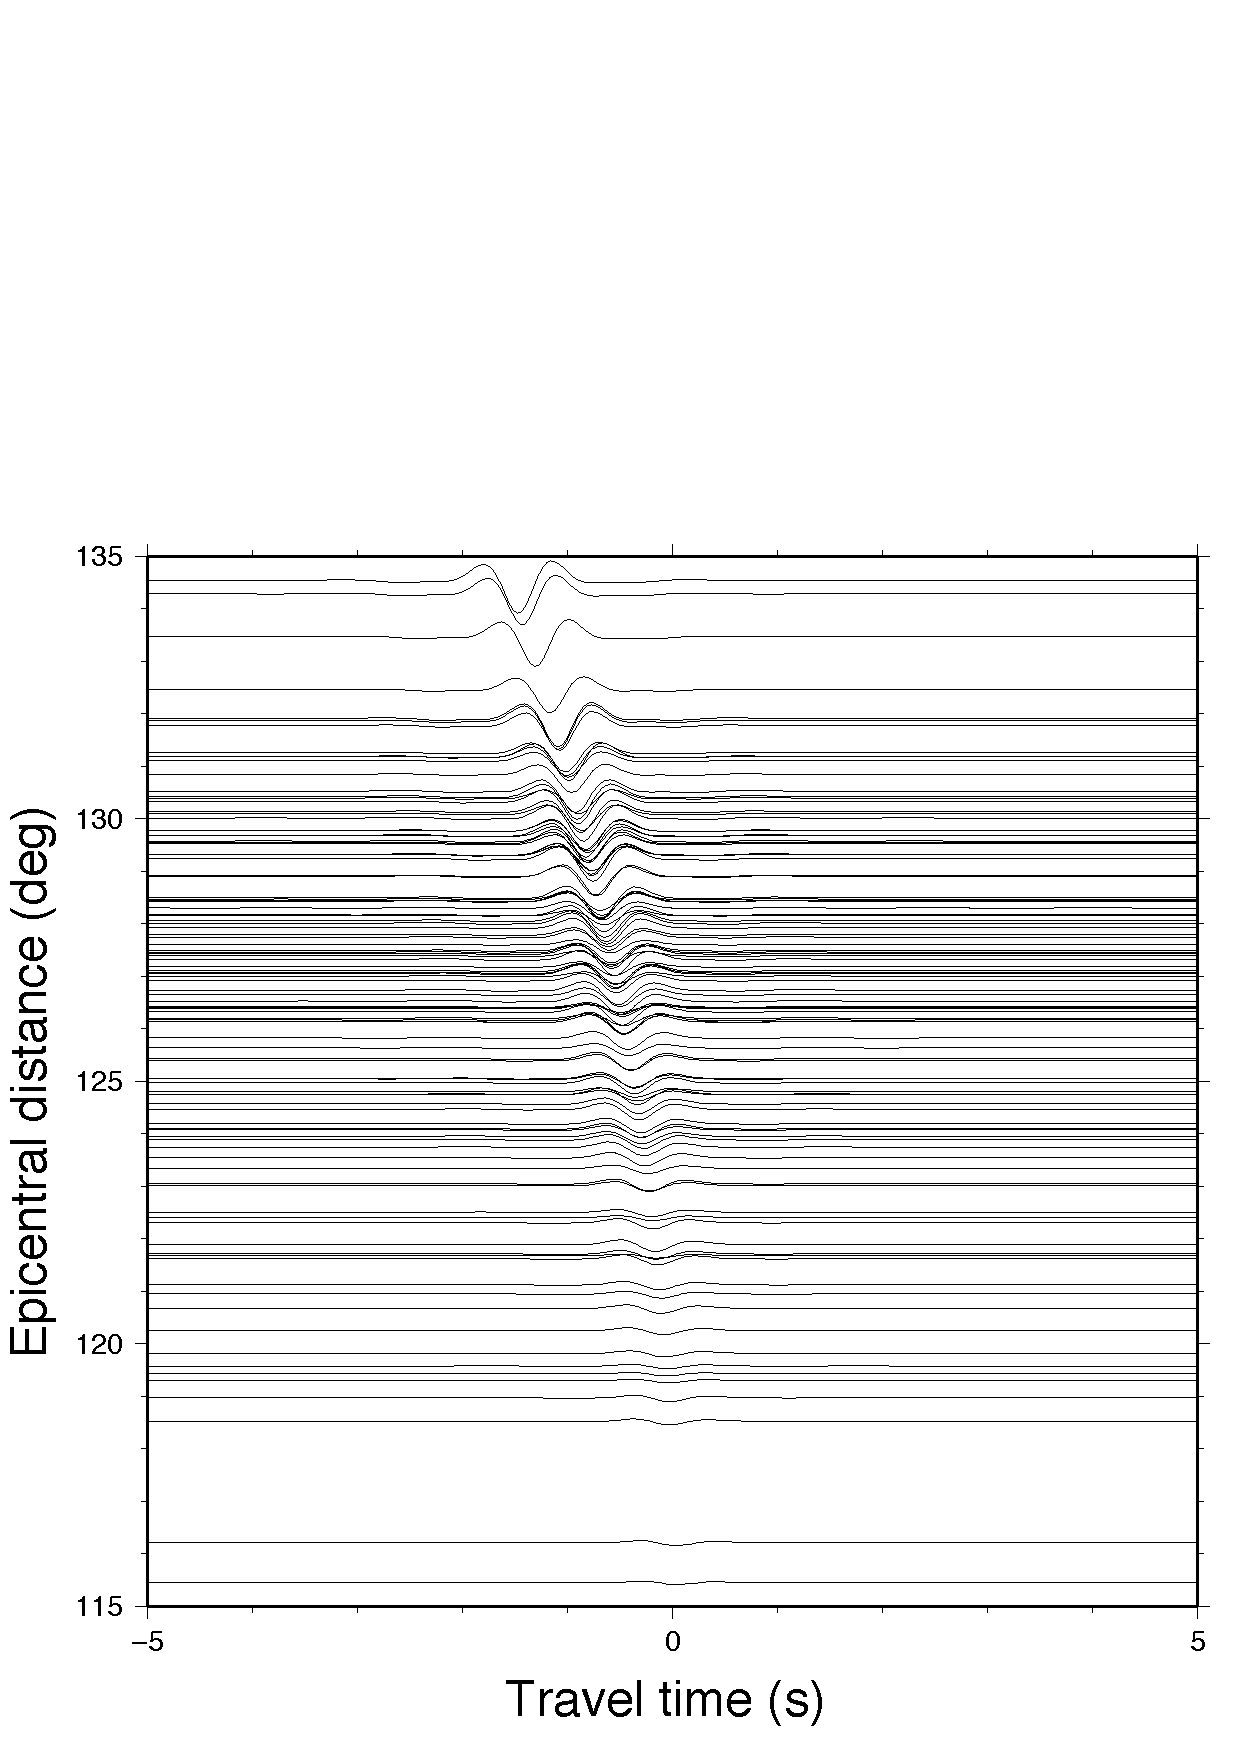
\includegraphics[width=0.4\textwidth]{figures/celebessea/celebessea_KIK_aligned}
	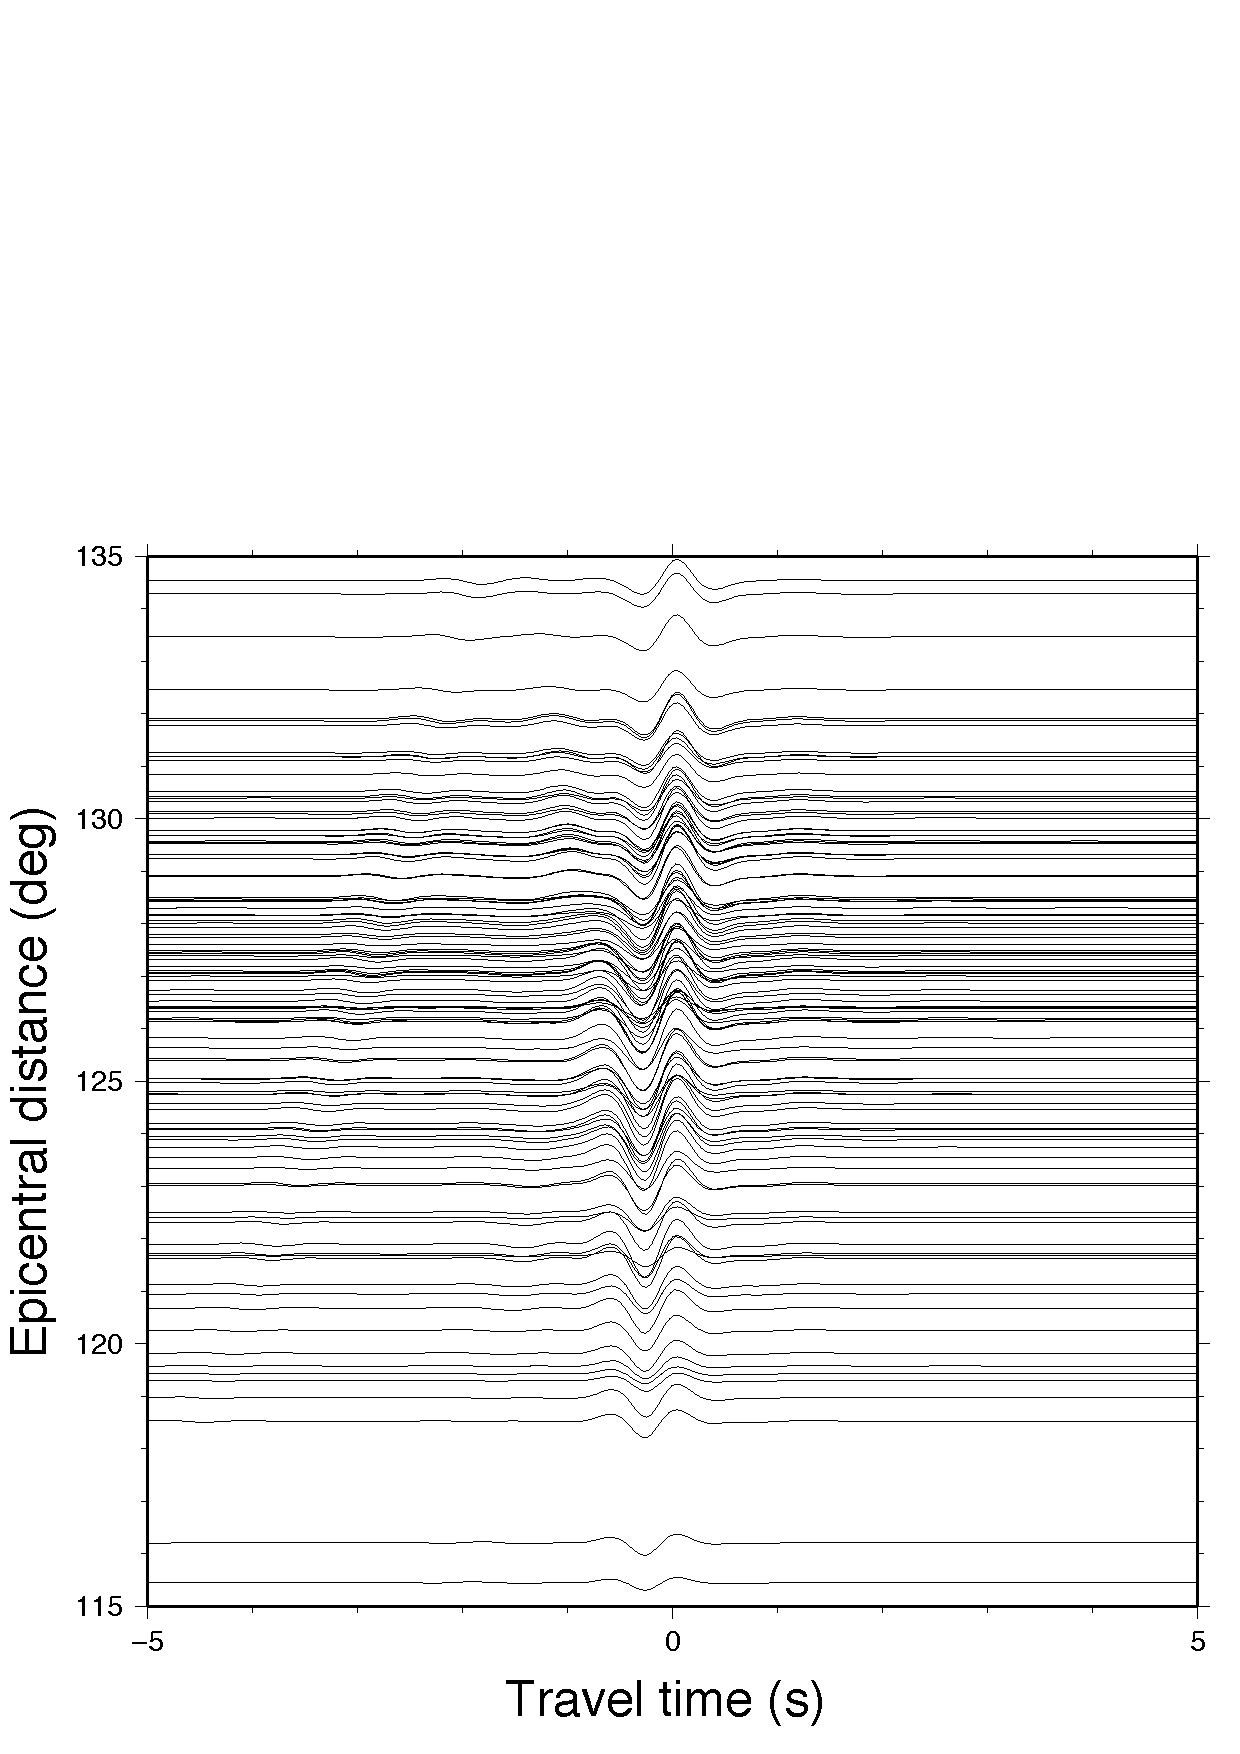
\includegraphics[width=0.4\textwidth]{figures/celebessea/celebessea_pkikp_aligned}
	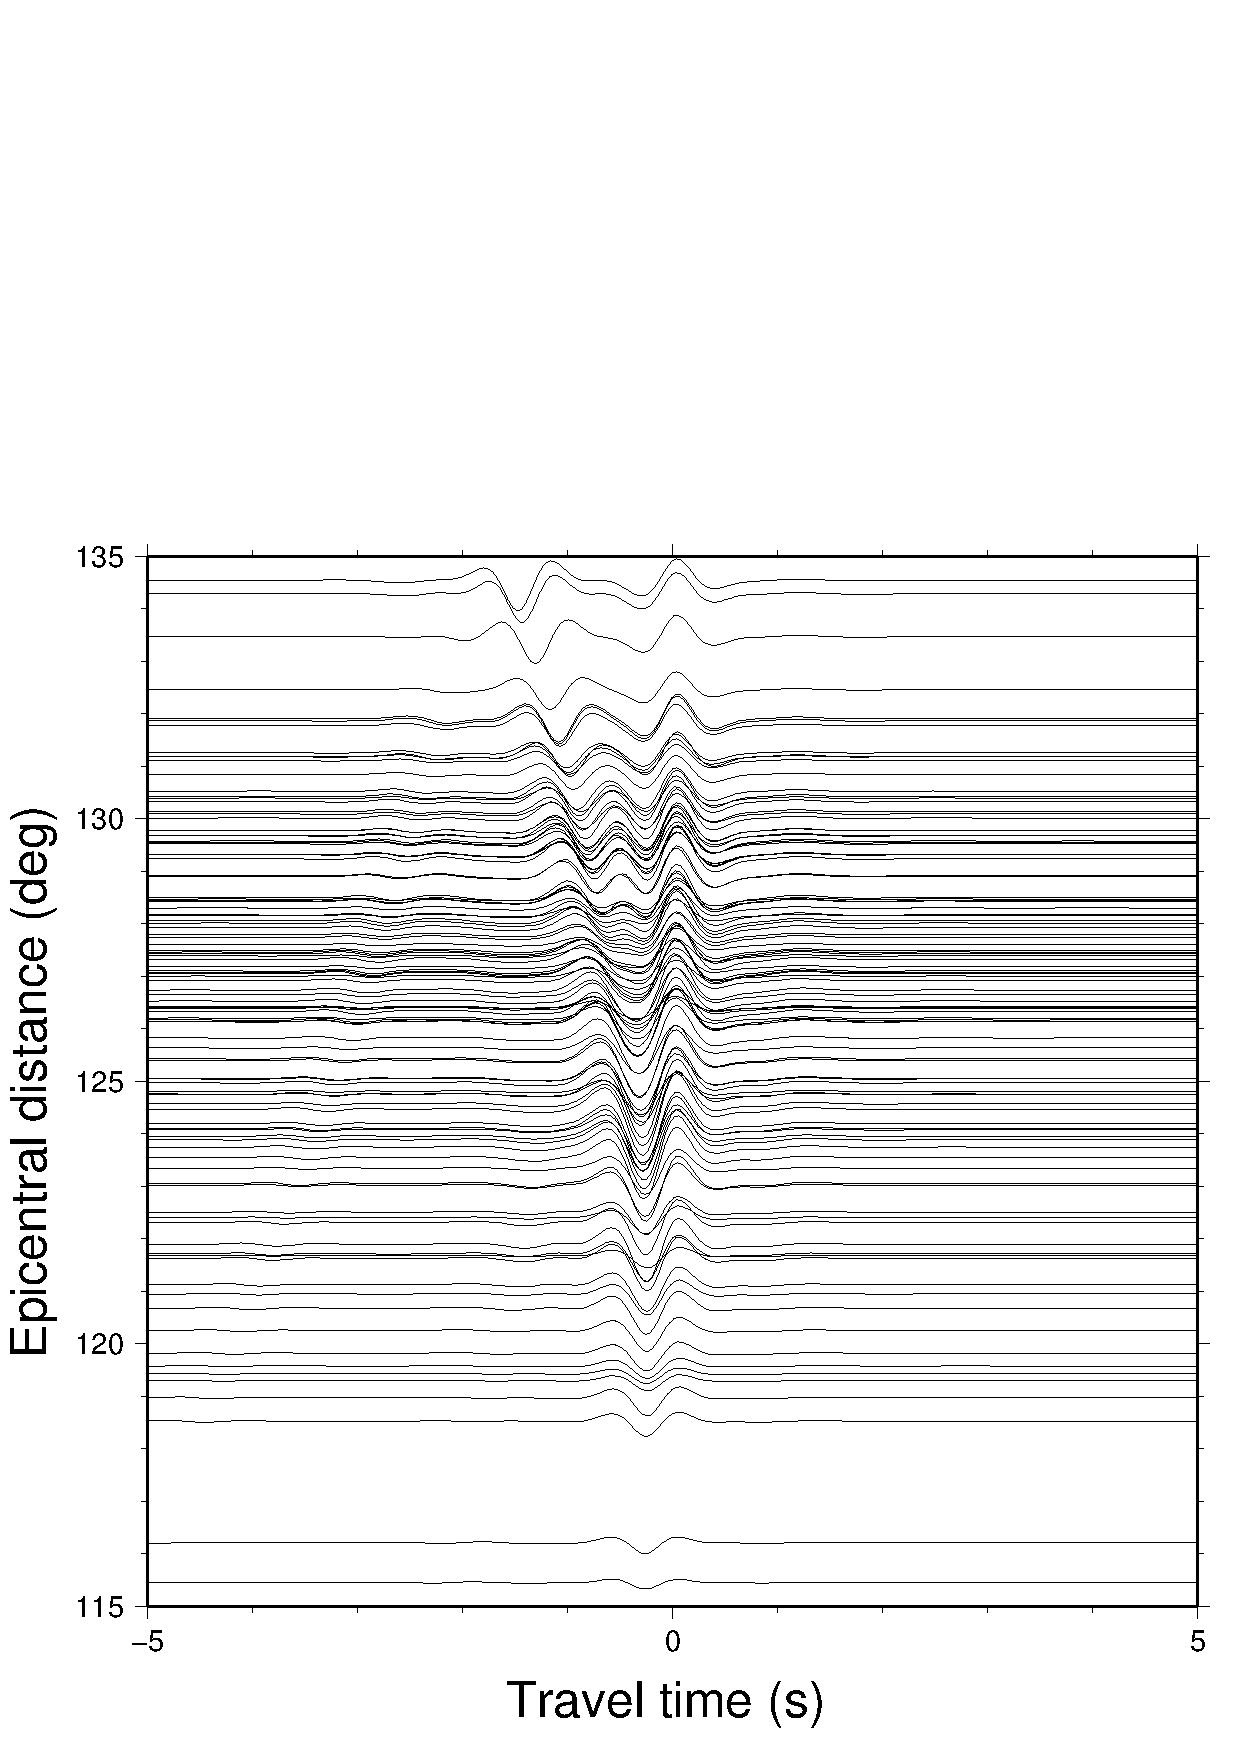
\includegraphics[width=0.4\textwidth]{figures/celebessea/celebessea_both_aligned}
	\caption{Separated PKIKP (top left) PKiKP (top right), and combined (bottom) synthetic seismograms for the Celebes Sea event.}
	\label{fig:Synth aligned}
\end{figure}

%%%%
\section{The limits of PKiKP-PKIKP travel time analysis}

In this section we seek to quantitively measure the limits of PKiKP-PKIKP travel time analysis when used to measure the velocity structure of the inner core. Previous studies have only measured up to epicentral distances where PKiKP and PKIKP are clearly separate phases; in this study we will attempt to study much lower epicentral distances. As such it will be useful to know where we can make reliable PKiKP-PKIKP measurements using synthetic data which mimics real world data.

\subsection{Inner core travel time variations}

The end goal of this study is to calculate velocity structure perturbations using equation \eqref{eq:Delta v}. In what follows it will therefore be useful to know how $t$, the time a PKIKP ray spends in the inner core, varies as a function and bottoming depth below the ICB. For shallow depths this is shown in figure \ref{fig:Time in core}. Although only data for an source depth of $\sim$100km is shown, we have plotted similar data for source depths in the range 30km - 575km to confirm that the data is not a function of source depth.

\begin{figure}
	\centering
	\includegraphics[width=0.7\textwidth]{figures/time_in_core}
	\caption{The time PKIKP spends in the inner core as a function of bottoming depth of the ray.}
	\label{fig:Time in core}
\end{figure}

The error in an individual velocity perturbation calculated using equation \eqref{eq:Delta v} is
\begin{equation}
	\Delta \delta v = \frac{v_{model}}{t} \left ( \Delta \delta t - \Delta t \frac{\delta t}{t} \right )
\end{equation}
where we have taken into account possible error in the inner core travel time, $\Delta t$.


The only two features that are measurable at all distances in the combined seismograms are the initial downswing and the final downswing (see figure \ref{fig:Synth aligned}). When making measurements of real data we want to be sure that we are measuring a PKIKP feature (initial upswing) and PKiKP feature (final upswing), and not two PKiKP features. Measuring two PKiKP phase features is more likely at lower epicentral distances due to the PKIKP phase getting weaker, and the PKiKP phase developing a large upswing to the left. Incorrectly measuring two PKiKP features would cause a systematic overestimate of the true difference between the two phases. We also note that this is not a problem for synthetic data, where we can take measurements from the individual PKIKP and PKiKP seismograms separately.

At low epicentral distances PKiKP is the dominant phase. This means that on the combined seismogram, the final downswing is an accurate measurement of a PKiKP feature. This is confirmed in figure PUT FIGURE HERE where we plot measurements of the initial downswing in the combined and PKiKP case at distances where PKiKP has a well defined initial downswing. The two data sets agree well to within errors, confirming our assertion that on combined seismograms the final downswing is always a PKiKP feature.

In contrast, the left downswing may not be an accurate measurement of a PKIKP feature at low epicentral distances. To quantify where measurements on the combined seismogram become inaccurate, we plot the difference between PKIKP initial downswings (see top left, figure \ref{fig:Synth aligned}) and combined initial downswing (see bottom, figure \ref{fig:Synth aligned}). On the same figure we also plot the difference between PKiKP initial downswings and PKIKP initial downswings. This data is shown in figure \ref{fig:Downswing differences}. A three point moving average is applied in order to smooth the data; this does not significantly change the distribution of data. At epicentral distances $< 127^{\circ}$ PKiKP and combined measurements coincide. We should therefore not trust measurements below $127^{\circ}$.

\begin{figure}
	\centering
	\includegraphics[width=0.7\textwidth]{figures/downswing_differences}
	\caption{Initial downswing measurements for PKiKP and combined synthetic seismograms. Measurements are taken relative to initial PKIKP downswings.}
	\label{fig:Downswing differences}
\end{figure}

\subsection{Effect of different velocity models}
Analysis in this section so far has used the spherically symmetric AK135 model to generate data. In the real world, however, deviations from this model of the order PUT VALUE AND REFERENCES HERE have been measured (\cite{Waszek2011a}, \cite{Yee2014}). We therefore carry out similar analysis using two different velocity models which are shown in figure PUT VELOCITY MODEL FIGURE HERE. In each case we perturb the P wave velocity at the ICB and keep all other parameters as in AK135. These models correspond to realistic eastern hemisphere and western hemisphere isotropic models, taken from \cite{Waszek2011a} and averaged over the top 60km of the inner core.

%%%%
\appendix
\section{Software details}
\label{app:Software}
The following lists the software used in this paper along with brief descriptions of what each piece of software was used for.
\begin{itemize}
	\item IRIS Wilber
	\begin{itemize}
		\item Used to select events and download worldwide seismic data from each selected event.
	\end{itemize}
	\item Centroid Moment Tensor (CMT) Catalogue
	\begin{itemize}
		\item Used to set earthquake time and location, and to feed WKBJ with resolved moment tensors on an event by event basis.
	\end{itemize}
	\item Matlab 2015a (8.5.0.197613, maci64)
\end{itemize}

%%%%
\newpage
% Bibliography
\bibliographystyle{agu}
\bibliography{/Users/dstansby/Physics/Papers/library}

\end{document}